% --------------------------------------------------
%  TALLER DE INTRODUCCIÓN A LaTeX
%  https://github.com/mianfg/latex-intro
%
%  Sesión 1 -> Presentación
%
%  Autor: Miguel Ángel Fernández Gutiérrez, @mianfg
%  Fecha: 20 febrero, 2019
% --------------------------------------------------

% Tipo de documento (presentación)
\documentclass[10pt, xcolor=table]{beamer}
\usepackage{caption}
\usepackage{subcaption}

\setcounter{MaxMatrixCols}{20}

% Cargar el tema
\usetheme{metropolis}

%  __________
% |          |
% | Paquetes |
% |__________|

% Paquetes de idioma
\usepackage[utf8]{inputenc}
\usepackage[spanish, es-tabla, es-lcroman, es-noquoting]{babel}

% Paquete para código fuente
% LISTINGS
\usepackage{listings}
\usepackage{lipsum}
\usepackage{courier}
\usepackage{csvsimple}
\usepackage{graphicx}
\newcommand{\scalemath}[2]{\scalebox{#1}{\begin{math} {#2} \end{math}}}

% Colores para los bloques de código
\definecolor{codegreen}{rgb}{0,0.6,0}
\definecolor{codegray}{rgb}{0.5,0.5,0.5}
\definecolor{codepurple}{rgb}{0.58,0,0.82}
\definecolor{backcolour}{rgb}{0.95,0.95,0.92}
\lstdefinestyle{mystyle}{
	backgroundcolor=\color{backcolour},   
	commentstyle=\color{codegreen},
	keywordstyle=\color{blue},
	numberstyle=\tiny\color{codegray},
	stringstyle=\color{codepurple},
	basicstyle=\footnotesize\ttfamily,
	breakatwhitespace=false,         
	breaklines=true,                 
	captionpos=b,                    
	keepspaces=true,                 
	numbers=left,                    
	numbersep=5pt,                  
	showspaces=false,                
	showstringspaces=false,
	showtabs=false,                  
	tabsize=4
}
\lstset{style=mystyle}

% Paquete de numeración en Beamer
\usepackage{appendixnumberbeamer}

% Paquete de uso para plantilla
\usepackage{booktabs}
\usepackage[scale=2]{ccicons}

% Paquete para controlar espacios
\usepackage{xspace}
\newcommand{\themename}{\textbf{\textsc{metropolis}}\xspace}

% Paquetes para matemáticas
\usepackage{amsmath}    % Paquete básico de matemáticas
\usepackage{amsthm}     % Teoremas
\usepackage{mathrsfs}   % Fuente para ciertas letras utilizadas en matemáticas

% Paquetes para fuentes
\usepackage{newpxtext, newpxmath}   % Fuente similar a Palatino
\usepackage{FiraSans}               % Fuente sans serif
\usepackage[T1]{fontenc}
\usepackage[italic]{mathastext}     % Utiliza la fuente del documento
                                    % en los entornos matemáticos

%  ________________________
% |                        |
% | Configuración del tema |
% |________________________|

% Configuración básica del tema
\metroset{
  % tema oscuro ('dark') o claro ('light'). No tiene efecto al usar la
  % paleta de colores más adelante
  background=light,
  % 'none' para eliminar la diapositiva inicial de cada sección
  sectionpage=progressbar,
  % 'progressbar' o 'simple' para añadir una diapositiva inicial a cada subsección
  subsectionpage=none,
  % contador de página: 'none', 'counter' o 'fraction'
  numbering=none,
  % barra de progreso: 'none', 'head', 'frametitle' o 'foot'
  progressbar=frametitle,
  % fondo de los bloques estilo teorema: 'transparent' o 'fill'
  block=fill,
}

% Paleta de colores
\definecolor{accent}{HTML}{009688}
\colorlet{darkaccent}{accent!70!black}
\definecolor{foreground}{RGB}{0, 0, 0}
\definecolor{background}{RGB}{255, 255, 255}

% Insertar los colores en el tema
\setbeamercolor{normal text}{fg=foreground, bg=background}
\setbeamercolor{alerted text}{fg=darkaccent, bg=background}
\setbeamercolor{example text}{fg=foreground, bg=background}
\setbeamercolor{frametitle}{fg=background, bg=accent}

\setbeamercolor{headtitle}{fg=background!70!accent,bg=accent!90!foreground}
\setbeamercolor{headnav}{fg=background,bg=accent!90!foreground}
\setbeamercolor{section in head/foot}{fg=background,bg=accent}

\defbeamertemplate*{headline}{miniframes theme no subsection}{
  % Caja para mostrar título y autor encima de cada diapositiva
  % Nosotros no 
  %% \begin{beamercolorbox}[ht=2.5ex,dp=1.125ex,
  %%     leftskip=.3cm,rightskip=.3cm plus1fil]{headtitle}
  %%   {\usebeamerfont{title in head/foot}\insertshorttitle}
  %%   \hfill
  %%   \leavevmode{\usebeamerfont{author in head/foot}\insertshortauthor}
  %% \end{beamercolorbox}
  %% \begin{beamercolorbox}[colsep=1.5pt]{upper separation line head}
  %% \end{beamercolorbox}

  % Caja para mostrar navegación encima de cada diapositiva
  \begin{beamercolorbox}{headnav}
    \vskip2pt\insertnavigation{\paperwidth}\vskip2pt
  \end{beamercolorbox}
  \begin{beamercolorbox}[colsep=1.5pt]{lower separation line head}
  \end{beamercolorbox}
}

%  _________
% |         |
% | Ajustes |
% |_________|

% Fijar tabla a posición
\usepackage{array}
\newcolumntype{L}[1]{>{\raggedright\let\newline\\\arraybackslash\hspace{0pt}}m{#1}}
\newcolumntype{C}[1]{>{\centering\let\newline\\\arraybackslash\hspace{0pt}}m{#1}}
\newcolumntype{R}[1]{>{\raggedleft\let\newline\\\arraybackslash\hspace{0pt}}m{#1}}

%  ________
% |        |
% | Título |
% |________|

\title{Programación Dinámica}
\subtitle{Algorítmica. \alert{Práctica 4}}
\date{Mayo 2022}
\author{Jose Alberto Hoces Castro\\Javier Gómez López\\ Manuel Moya Martín Castaño\\[4pt]}
\titlegraphic{\hfill
\includegraphics[width=2.5cm]{logo_dark.jpg}}

%  ___________
% |           |
% | Documento |
% |___________|

\begin{document}
\maketitle

\begin{frame}{Contenidos}
	\setbeamertemplate{section in toc}[sections numbered]
	\tableofcontents[]
\end{frame}

\begin{frame}[fragile]{Objetivo de la práctica}
	El objetivo de esta práctica es aprender a implementar y utilizar algoritmos que utilizan la técnica de programación dinámica. Para ello hemos tenido que resolver el siguiente ejercicio:
\end{frame}

\section{Introducción}
\begin{frame}[fragile]{Enunciado}
Dos hermanos fueron separados al nacer y mediante un programa de televisión se han enterado que podrían ser hermanos. Ante esto, los dos están de acuerdo en hacerse un test de ADN para verificar si realmente son hermanos.
\end{frame}

\begin{frame}[fragile]{Enunciado}
Dadas las 2 entradas:\\

\textbf{PRIMERA} \\
Hermano 1 - abbcdefabcdxzyccd \\
Hermano 2 - abbcdeafbcdzxyccd \\

\textbf{SEGUNDA}\\
Hermano 1 - $010111000100010101010010001001001001$\\
Hermano 2 - $110000100100101010001010010011010100$\\

	\begin{itemize}
		\item Deben encontrar el \% de similitud que existe entre estos posibles hermanos, como es un ejemplo lo haremos para 2 entradas posibles.
		\item Dar las salidas (secuencia más larga) de las 2 entradas.
		\item Dar la matriz de los cálculos de la primera entrada.
	\end{itemize}

\end{frame}

\section{Requisitos de la programación dinámica}
\begin{frame}[fragile]{Requisitos de la Programación Dinámica}
	\begin{itemize}
		\item \textbf{Naturaleza n-etápica}
		\item \textbf{Verificación del POB (Principio de Optimalidad de Bellman)}
		\item \textbf{Planteamiento de una recurrencia}
	\end{itemize}
\end{frame}

\begin{frame}[fragile]{Requisitos de la Programación Dinámica. \normalfont{Recurrencia planteada}}
	1. Comenzaremos rellenando la primera fila y la primera columna de ceros.
	
	2. Rellenamos el resto de la matriz según el siguiente criterio:
	
\[
	A(i,j)= \left\{ \begin{array}{lcc}
		0 &   si  &  \hspace{0.2cm} i=j=0 \\
		\\ max(A(i-1,j),A(i,j-1)) &  si  & x_i \neq y_j \hspace{0.2cm}\\
		\\ A(i-1,j-1) + 1 & si & x_i = y_j \hspace{0.2cm}
	\end{array}
	\right.
	\]
	
	3. Por último, hallamos el máximo de la matriz (que estará situado en la última fila) deshaciendo el camino que hemos ido haciendo por las casillas y teniendo en cuenta si estamos en una posición de coincidencia o no.
\end{frame}

	
\begin{frame}[fragile]{Requisitos de la Programación Dinámica. \normalfont{Ejemplo}}
	Dado un ejemplo pequeño de secuencias, sean $<A,B,C,B,D,A,B>$ y $<B,D,C,A,B,A,E>$, la matriz usando nuestro algoritmo quedaría así:
	
	\begin{center}
		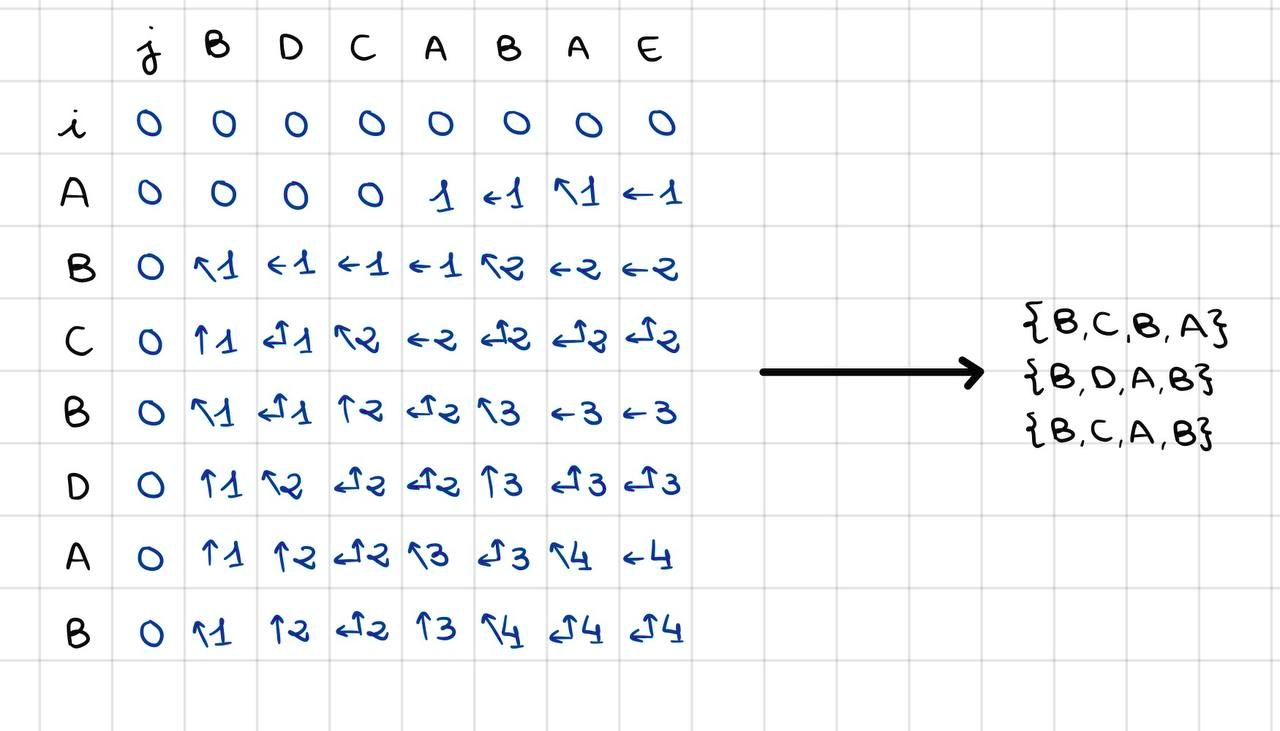
\includegraphics[scale=0.23]{./Ejemplo.png}
	\end{center}
\end{frame}


\begin{frame}[fragile]{Requisitos de la PD. \normalfont{Cálculo de una solución}}
	\textbf{1. Cálculo de la matriz}
	\lstinputlisting[language=C++]{./Code/calculo.cpp}
\end{frame}

\begin{frame}[fragile]{Requisitos de la PD. \normalfont{Cálculo de una solución}}
	\textbf{2. Localización del máximo y obtención de la subsecuencia más larga}
	\lstinputlisting[language=C++]{./Code/maxysub.cpp}
\end{frame}

\begin{frame}[fragile]{Requisitos de la PD. \normalfont{Cálculo de una solución}}
	\textbf{2. Localización del máximo y obtención de la subsecuencia más larga}
	\lstinputlisting[language=C++]{./Code/maxysub2.cpp}
\end{frame}


\section{Solución}
\begin{frame}[fragile]{Solución. \normalfont{Secuencias más largas}}
		\begin{center}
			SECUENCIA MÁS LARGA LETRAS: 
			\[
			a b b c d e a b c d z y c c d
			\]
			
			SECUENCIA MÁS LARGA NÚMEROS: 
			\[
			1 1 0 0 0 0 0 0 1 0 1 0 1 0 1 0 0 1 0 0 0 1 0 0 1 0 0 1 0 0
			\]
		\end{center}
\end{frame}

\begin{frame}[fragile]{Solución. \normalfont{Similitud}}

		\begin{center}
			PORCENTAJE DE SIMILITUD LETRAS: 88.2353\%
			
			PORCENTAJE DE SIMILITUD NÚMEROS: 83.3333\%
		\end{center}
\end{frame}

\begin{frame}[fragile]{Solución. \normalfont{Matriz de cálculos del primer problema}}
	\[
	\scalemath{0.7}{	
	\begin{matrix}
      &   & a & b & b & c & d & e & a & f & b & c & d & z & x & y & c & c & d \\
      & 0 & 0 & 0 & 0 & 0 & 0 & 0 & 0 & 0 & 0 & 0 & 0 & 0 & 0 & 0 & 0 & 0 & 0 \\
    a & 0 & 1 & 1 & 1 & 1 & 1 & 1 & 1 & 1 & 1 & 1 & 1 & 1 & 1 & 1 & 1 & 1 & 1 \\
    b & 0 & 1 & 2 & 2 & 2 & 2 & 2 & 2 & 2 & 2 & 2 & 2 & 2 & 2 & 2 & 2 & 2 & 2 \\
    b & 0 & 1 & 2 & 3 & 3 & 3 & 3 & 3 & 3 & 3 & 3 & 3 & 3 & 3 & 3 & 3 & 3 & 3 \\
    c & 0 & 1 & 2 & 3 & 4 & 4 & 4 & 4 & 4 & 4 & 4 & 4 & 4 & 4 & 4 & 4 & 4 & 4 \\
    d & 0 & 1 & 2 & 3 & 4 & 5 & 5 & 5 & 5 & 5 & 5 & 5 & 5 & 5 & 5 & 5 & 5 & 5 \\
    e & 0 & 1 & 2 & 3 & 4 & 5 & 6 & 6 & 6 & 6 & 6 & 6 & 6 & 6 & 6 & 6 & 6 & 6 \\
    f & 0 & 1 & 2 & 3 & 4 & 5 & 6 & 6 & 7 & 7 & 7 & 7 & 7 & 7 & 7 & 7 & 7 & 7 \\
    a & 0 & 1 & 2 & 3 & 4 & 5 & 6 & 7 & 7 & 7 & 7 & 7 & 7 & 7 & 7 & 7 & 7 & 7 \\
    b & 0 & 1 & 2 & 3 & 4 & 5 & 6 & 7 & 7 & 8 & 8 & 8 & 8 & 8 & 8 & 8 & 8 & 8 \\
    c & 0 & 1 & 2 & 3 & 4 & 5 & 6 & 7 & 7 & 8 & 9 & 9 & 9 & 9 & 9 & 9 & 9 & 9 \\
    d & 0 & 1 & 2 & 3 & 4 & 5 & 6 & 7 & 7 & 8 & 9 & 10 & 10 & 10 & 10 & 10 & 10 & 10  \\
    x & 0 & 1 & 2 & 3 & 4 & 5 & 6 & 7 & 7 & 8 & 9 & 10 & 10 & 11 & 11 & 11 & 11 & 11\\
    z & 0 & 1 & 2 & 3 & 4 & 5 & 6 & 7 & 7 & 8 & 9 & 10 & 11 & 11 & 11 & 11 & 11 & 11 \\
    y & 0 & 1 & 2 & 3 & 4 & 5 & 6 & 7 & 7 & 8 & 9 & 10 & 11 & 11 & 12 & 12 & 12 & 12\\
    c & 0 & 1 & 2 & 3 & 4 & 5 & 6 & 7 & 7 & 8 & 9 & 10 & 11 & 11 & 12 & 13 & 13 & 13 \\
    c & 0 & 1 & 2 & 3 & 4 & 5 & 6 & 7 & 7 & 8 & 9 & 10 & 11 & 11 & 12 & 13 & 14 & 14 \\
    d & 0 & 1 & 2 & 3 & 4 & 5 & 6 & 7 & 7 & 8 & 9 & 10 & 11 & 11 & 12 & 13 & 14 & 15 
	\end{matrix}
	}
	\]
\end{frame}

\section{Conclusiones}
\begin{frame}[fragile]{Conclusiones}
	\begin{itemize}
		\item Si hubiésemos resuelto este problema usando la \textbf{fuerza bruta}, es decir, enumerando todas las subsecuencias comunes existentes, obtendríamos un algoritmo de orden $O(d^n)$, siendo $d$ la longitud de las cadenas.
		\item Gracias a la \textbf{programación dinámica}, evitamos muchos de los cálculos que se harían en \textbf{fuerza bruta}, obteniendo así un algoritmo de \textbf{orden polinomial}, en este caso concretamente $O(n \cdot m)$, siendo $n$ y $m$ las longitudes de las secuencias de entrada.
	\end{itemize}
\end{frame}

\begin{frame}[fragile]{Conclusiones}
	\begin{itemize}
		\item Obtenemos la \textbf{solución optimal}, cosa que no habríamos logrado con otras técnicas ya vistas como \textbf{Greedy}
	\item También ganamos ventaja respecto a \textbf{Divide y Vencerás}, pues en \textbf{programación dinámica} tenemos problemas que están \textbf{encajados}, por lo que \textbf{no repetimos cálculos}.
	\item Como principal \textbf{inconveniente} de la \textbf{programación dinámica}, se hace un \textbf{gran uso de recursos}, en nuestro caso, la \textbf{memoria} reservada para nuestra \textbf{matriz de cálculos}.
	\end{itemize}
\end{frame}


\end{document}